\documentclass[tikz,border=5pt]{standalone}
\usetikzlibrary{calc}
\begin{document}
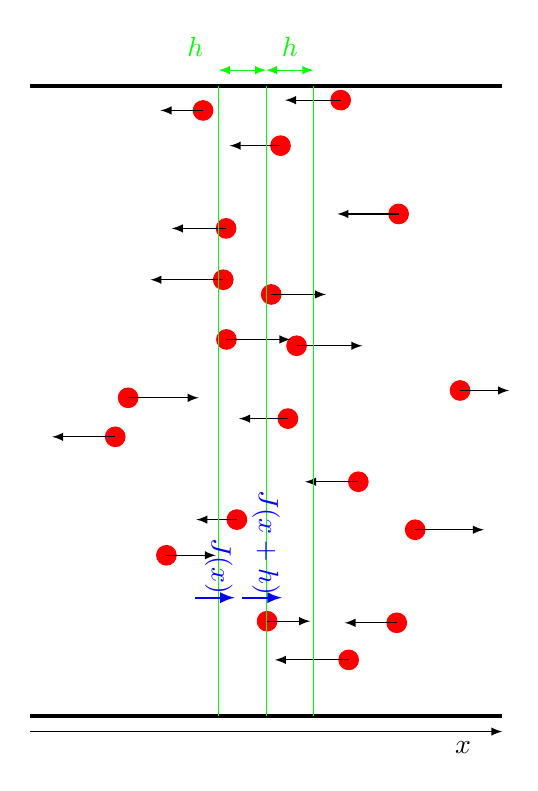
\begin{tikzpicture}
\draw[-,ultra thick] (4,0)--(10,0) ;
\draw[-,ultra thick] (4,8)--(10,8) ;

\draw[-latex] (4,-0.2)--(10,-0.2) ;
\node[] at (9.5,-0.4) {$x$};


\coordinate (a) at (6.1992534,7.687872);
\node[circle, draw=red, fill=red,minimum size=0.1,inner sep=2.5] at (a) {};
\draw[-latex] ($ (a) + (0,0) $) -- ($ (a) + (-0.54099618,0) $);

\coordinate (a) at (7.38701,4.69941);
\node[circle, draw=red, fill=red,minimum size=0.1,inner sep=2.5] at (a) {};
\draw[-latex] ($ (a) + (0,0) $) -- ($ (a) + (0.836021,0) $);

\coordinate (a) at (7.01255,1.2013);
\node[circle, draw=red, fill=red,minimum size=0.1,inner sep=2.5] at (a) {};
\draw[-latex] ($ (a) + (0,0) $) -- ($ (a) + (0.54883,0) $);

\coordinate (a) at ( 5.0836,3.54286);
\node[circle, draw=red, fill=red,minimum size=0.1,inner sep=2.5] at (a) {};
\draw[-latex] ($ (a) + (0,0) $) -- ($ (a) + (-0.80153,0) $);

\coordinate (a) at ( 9.46324,4.13163);
\node[circle, draw=red, fill=red,minimum size=0.1,inner sep=2.5] at (a) {};
\draw[-latex] ($ (a) + (0,0) $) -- ($ (a) + (0.6223,0) $);

\coordinate (a) at (8.1714,2.97226);
\node[circle, draw=red, fill=red,minimum size=0.1,inner sep=2.5] at (a) {};
\draw[-latex] ($ (a) + (0,0) $) -- ($ (a) + (-0.67755,0) $);

\coordinate (a) at (5.24745,4.038505);
\node[circle, draw=red, fill=red,minimum size=0.1,inner sep=2.5] at (a) {};
\draw[-latex] ($ (a) + (0,0) $) -- ($ (a) + (0.89719,0) $);

\coordinate (a) at (8.65917,1.181025);
\node[circle, draw=red, fill=red,minimum size=0.1,inner sep=2.5] at (a) {};
\draw[-latex] ($ (a) + (0,0) $) -- ($ (a) + (-0.66351,0) $);

\coordinate (a) at (6.62881,2.491796);
\node[circle, draw=red, fill=red,minimum size=0.1,inner sep=2.5] at (a) {};
\draw[-latex] ($ (a) + (0,0) $) -- ($ (a) + (-0.51517,0) $);

\coordinate (a) at (5.733701,2.038457);
\node[circle, draw=red, fill=red,minimum size=0.1,inner sep=2.5] at (a) {};
\draw[-latex] ($ (a) + (0,0) $) -- ($ (a) + (0.62819,0) $);






\coordinate (a) at (8.68277907,6.37325);
\node[circle, draw=red, fill=red,minimum size=0.1,inner sep=2.5] at (a) {};
\draw[-latex] ($ (a) + (0,0) $) -- ($ (a) + (-0.7780672,0) $);

\coordinate (a) at (6.495950,4.77974);
\node[circle, draw=red, fill=red,minimum size=0.1,inner sep=2.5] at (a) {};
\draw[-latex] ($ (a) + (0,0) $) -- ($ (a) + (0.81444,0) $);

\coordinate (a) at (7.1826,7.240460);
\node[circle, draw=red, fill=red,minimum size=0.1,inner sep=2.5] at (a) {};
\draw[-latex] ($ (a) + (0,0) $) -- ($ (a) + (-0.64647,0) $);

\coordinate (a) at (7.9470,7.818810);
\node[circle, draw=red, fill=red,minimum size=0.1,inner sep=2.5] at (a) {};
\draw[-latex] ($ (a) + (0,0) $) -- ($ (a) + (-0.70764,0) $);

\coordinate (a) at (8.04827,0.710135);
\node[circle, draw=red, fill=red,minimum size=0.1,inner sep=2.5] at (a) {};
\draw[-latex] ($ (a) + (0,0) $) -- ($ (a) + (-0.937509,0) $);

\coordinate (a) at (7.0648,5.351072);
\node[circle, draw=red, fill=red,minimum size=0.1,inner sep=2.5] at (a) {};
\draw[-latex] ($ (a) + (0,0) $) -- ($ (a) + (0.6957202,0) $);

\coordinate (a) at (6.45560,5.5380827);
\node[circle, draw=red, fill=red,minimum size=0.1,inner sep=2.5] at (a) {};
\draw[-latex] ($ (a) + (0,0) $) -- ($ (a) + (-0.925299,0) $);

\coordinate (a) at (8.893164,2.3627631);
\node[circle, draw=red, fill=red,minimum size=0.1,inner sep=2.5] at (a) {};
\draw[-latex] ($ (a) + (0,0) $) -- ($ (a) + (0.8736058,0) $);

\coordinate (a) at (6.491792,6.18976);
\node[circle, draw=red, fill=red,minimum size=0.1,inner sep=2.5] at (a) {};
\draw[-latex] ($ (a) + (0,0) $) -- ($ (a) + (-0.690002,0) $);

\coordinate (a) at (7.2765842,3.7742630);
\node[circle, draw=red, fill=red,minimum size=0.1,inner sep=2.5] at (a) {};
\draw[-latex] ($ (a) + (0,0) $) -- ($ (a) + (-0.620690,0) $);





\draw[-,green] (6.4,0) -- (6.4,8);
\draw[-,green] (7,0) -- (7,8);
\draw[-,green] (7.6,0) -- (7.6,8);


%\node[green, rotate=-90] at (6.7,-0.5) {$x$};
%\node[green, rotate=-90] at (7.3,-0.8) {$x+h$};

\draw[latex-latex,green] (6.4,8.2) -- (7,8.2);
\node[green] at (6.1,8.5) {$h$};

\draw[latex-latex,green] (7,8.2) -- (7.6,8.2);
\node[green] at (7.3,8.5) {$h$};

\draw[-latex,blue,thick] (6.1,1.5) -- (6.6,1.5);
\node[blue,rotate=-90] at (6.4,1.9) {$J(x)$};

\draw[-latex,blue,thick] (6.7,1.5) -- (7.2,1.5);
\node[blue,rotate=-90] at (7,2.2) {$J(x+h)$};


\end{tikzpicture}
\end{document}